\PassOptionsToPackage{unicode=true}{hyperref} % options for packages loaded elsewhere
\PassOptionsToPackage{hyphens}{url}
%
\documentclass[]{book}
\usepackage{lmodern}
\usepackage{amssymb,amsmath}
\usepackage{ifxetex,ifluatex}
\usepackage{fixltx2e} % provides \textsubscript
\ifnum 0\ifxetex 1\fi\ifluatex 1\fi=0 % if pdftex
  \usepackage[T1]{fontenc}
  \usepackage[utf8]{inputenc}
  \usepackage{textcomp} % provides euro and other symbols
\else % if luatex or xelatex
  \usepackage{unicode-math}
  \defaultfontfeatures{Ligatures=TeX,Scale=MatchLowercase}
\fi
% use upquote if available, for straight quotes in verbatim environments
\IfFileExists{upquote.sty}{\usepackage{upquote}}{}
% use microtype if available
\IfFileExists{microtype.sty}{%
\usepackage[]{microtype}
\UseMicrotypeSet[protrusion]{basicmath} % disable protrusion for tt fonts
}{}
\IfFileExists{parskip.sty}{%
\usepackage{parskip}
}{% else
\setlength{\parindent}{0pt}
\setlength{\parskip}{6pt plus 2pt minus 1pt}
}
\usepackage{hyperref}
\hypersetup{
            pdftitle={Applet Codebook: CA Partners Daily MindLogger Diary v0.1},
            pdfauthor={Mike X.},
            pdfborder={0 0 0},
            breaklinks=true}
\urlstyle{same}  % don't use monospace font for urls
\usepackage{longtable,booktabs}
% Fix footnotes in tables (requires footnote package)
\IfFileExists{footnote.sty}{\usepackage{footnote}\makesavenoteenv{longtable}}{}
\usepackage{graphicx,grffile}
\makeatletter
\def\maxwidth{\ifdim\Gin@nat@width>\linewidth\linewidth\else\Gin@nat@width\fi}
\def\maxheight{\ifdim\Gin@nat@height>\textheight\textheight\else\Gin@nat@height\fi}
\makeatother
% Scale images if necessary, so that they will not overflow the page
% margins by default, and it is still possible to overwrite the defaults
% using explicit options in \includegraphics[width, height, ...]{}
\setkeys{Gin}{width=\maxwidth,height=\maxheight,keepaspectratio}
\setlength{\emergencystretch}{3em}  % prevent overfull lines
\providecommand{\tightlist}{%
  \setlength{\itemsep}{0pt}\setlength{\parskip}{0pt}}
\setcounter{secnumdepth}{5}
% Redefines (sub)paragraphs to behave more like sections
\ifx\paragraph\undefined\else
\let\oldparagraph\paragraph
\renewcommand{\paragraph}[1]{\oldparagraph{#1}\mbox{}}
\fi
\ifx\subparagraph\undefined\else
\let\oldsubparagraph\subparagraph
\renewcommand{\subparagraph}[1]{\oldsubparagraph{#1}\mbox{}}
\fi

% set default figure placement to htbp
\makeatletter
\def\fps@figure{htbp}
\makeatother

\usepackage{booktabs}
\usepackage[]{natbib}
\bibliographystyle{apalike}

\title{Applet Codebook: CA Partners Daily MindLogger Diary v0.1}
\author{Mike X.}
\date{2020-09-15}

\begin{document}
\maketitle

{
\setcounter{tocdepth}{1}
\tableofcontents
}
\hypertarget{part-protocol-intro}{%
\part{Protocol Intro}\label{part-protocol-intro}}

\hypertarget{intro}{%
\chapter*{Intro To Protocol (IN PROGRESS)}\label{intro}}
\addcontentsline{toc}{chapter}{Intro To Protocol (IN PROGRESS)}

\hypertarget{ca-partners-daily-mindlogger-diary}{%
\section{CA Partners Daily MindLogger Diary}\label{ca-partners-daily-mindlogger-diary}}

\ldots{}add info about the applet here\ldots{}

\hypertarget{part-protocol-codebook}{%
\part{Protocol Codebook}\label{part-protocol-codebook}}

\hypertarget{teen_section}{%
\chapter{Teen Self Report}\label{teen_section}}

\hypertarget{morning_bedtime}{%
\section{morning\_bedtime}\label{morning_bedtime}}

\textbf{Question}: ``About what time did you go to bed last night (regardless of the time you actually fell asleep)?''

\textbf{Visibility}: \emph{Always}

\textbf{Item Type}: Time input

\textbf{Header Image}:

\begin{flushleft}
\includegraphics[width=0.33\linewidth]{downloadFigs4latex_ca_partners_applet_codebook/morning_bedtime_headerImg} \end{flushleft}

\textbf{Responses}: \emph{Time in HH:MM AM/PM format via clock widget}

\hypertarget{morning_sleep_quality}{%
\section{morning\_sleep\_quality}\label{morning_sleep_quality}}

\textbf{Question}: ``How did you sleep last night?''

\textbf{Visibility}: \emph{Always}

\textbf{Item Type}: Slider bar

\textbf{Header Image}: \emph{None}

\textbf{Responses}:

Value

Label

Image

1

very poor

2

2

3

3

4

4

5

5

6

6

7

very good

\hypertarget{screen_after_bedtime}{%
\section{screen\_after\_bedtime}\label{screen_after_bedtime}}

\textbf{Question}: ``How much time was there between looking at a screen (cell phone, tv, computer, tablet, laptop) and going to sleep last night?''

\textbf{Visibility}: \emph{Always}

\textbf{Item Type}: Single-select radio button

\textbf{Header Image}:

\begin{flushleft}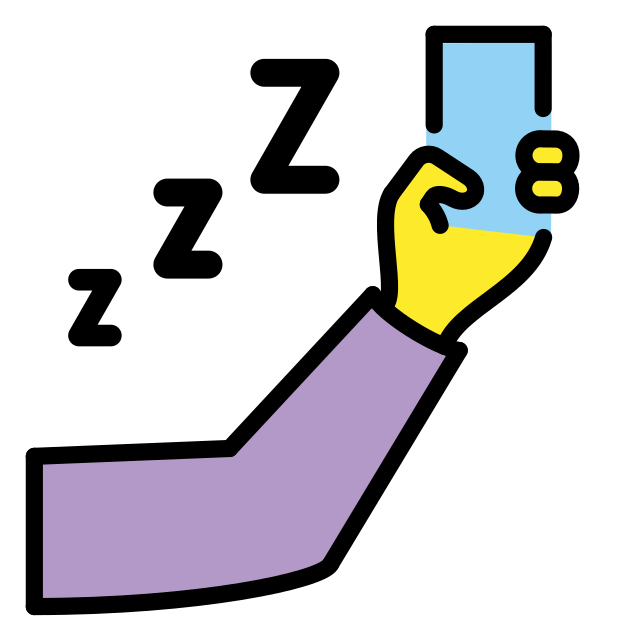
\includegraphics[width=0.33\linewidth]{downloadFigs4latex_ca_partners_applet_codebook/screen_after_bedtime_headerImg} \end{flushleft}

\textbf{Responses}:

Value

Label

0

0 hours (Turning a screen off was the last thing you did before falling asleep. Also includes falling asleep with the screen on.)

1

1/2 hour or less

2

1 hour

3

1-2 hours

4

2-4 hours

5

4-6 hours

6

6-8 hours

\hypertarget{socialmedia_fall_asleep}{%
\section{socialmedia\_fall\_asleep}\label{socialmedia_fall_asleep}}

\textbf{Question}: ``Did your use of social media impact your ability to fall asleep last night?''

\textbf{Visibility}: \emph{Always}

\textbf{Item Type}: Single-select radio button

\textbf{Header Image}:

\begin{flushleft}
\includegraphics[width=0.33\linewidth]{downloadFigs4latex_ca_partners_applet_codebook/socialmedia_fall_asleep_headerImg} \end{flushleft}

\textbf{Responses}:

Value

Label

1

Yes

0

No

\hypertarget{phone_location}{%
\section{phone\_location}\label{phone_location}}

\textbf{Question}: ``Where was your phone last night while you slept?''

\textbf{Visibility}: \emph{Always}

\textbf{Item Type}: Single-select radio button

\textbf{Header Image}: \emph{None}

\textbf{Responses}:

Value

Label

1

On my bed

2

In my room

3

In my room but I couldn't reach it without getting out of bed

4

In my room but turned off

5

Outside of my room

\hypertarget{school_device}{%
\section{school\_device}\label{school_device}}

\textbf{Question}: ``If you had school today, online or in-person, did you multitask on devices during classes?''

\textbf{Visibility}: \emph{Always}

\textbf{Item Type}: Single-select radio button

\textbf{Header Image}: \emph{None}

\textbf{Responses}:

Value

Label

1

I didn't have school today

2

Yes

3

No

\hypertarget{school_device_activity}{%
\section{school\_device\_activity}\label{school_device_activity}}

\textbf{Question}: ``If yes, what were you doing on your devices during class? (select all that apply)''

\textbf{Visibility}: \protect\hyperlink{school_device}{school\_device} = 2

\textbf{Item Type}: Multi-select checkbox

\textbf{Header Image}: \emph{None}

\textbf{Responses}:

Value

Label

1

Checking Instagram

2

Posting on Instagram

3

Watching TikToks

4

Making a TikTok

5

Checking Snapchat

6

Posting on Snapchat

7

Facetiming

8

Texting

9

Playing a game

10

Online Shopping

11

Doing work from another class

12

Other

\hypertarget{school_device_activity_other}{%
\section{school\_device\_activity\_other}\label{school_device_activity_other}}

\textbf{Question}: ``What \emph{other} activity were you doing on your device?''

\textbf{Visibility}: \protect\hyperlink{school_device_activity}{school\_device\_activity}.includes(12)

\textbf{Item Type}:

\textbf{Header Image}: \emph{None}

\textbf{Responses}: \emph{This item is text response}

\hypertarget{physical_activity}{%
\section{physical\_activity}\label{physical_activity}}

\textbf{Question}: ``Please select the intensity level of activities you did today:''

\textbf{Visibility}: \emph{Always}

\textbf{Item Type}: Multi-select checkbox

\textbf{Header Image}: \emph{None}

\textbf{Responses}:

Value

Label

Image

1

vigorous activities (e.g.~running/fast cycling/heavy lifting or digging)

2

moderate activities (e.g.~tennis/bicycling/carrying light loads)

3

light activities (e.g.~walking/climbing stairs/routine household chores)

4

No physical activity today

\hypertarget{internet_use_category}{%
\section{internet\_use\_category}\label{internet_use_category}}

\textbf{Question}: ``What did you use the internet for today?''

\textbf{Visibility}: \emph{Always}

\textbf{Item Type}: Multi-select checkbox

\textbf{Header Image}: \emph{None}

\textbf{Responses}:

Value

Label

1

Chat rooms/Group chat

2

Facetime/Video chat app

3

Blogs/Vlogs/Youtube

4

Music (Spotify/iTunes/etc.)

5

News

6

Direct messenger/texting

7

Gaming

8

Shopping

9

Social Networking (Snapchat/Instagram/TikTok/etc.)

10

Web browsing

11

Internet TV (Hulu/Amazon Prime/Netflix/etc.)

12

School/work

\hypertarget{social_media_duration}{%
\section{social\_media\_duration}\label{social_media_duration}}

\textbf{Question}: ``How many hours did you spend on social media today?''

\textbf{Visibility}: \emph{Always}

\textbf{Item Type}: Single-select radio button

\textbf{Header Image}: \emph{None}

\textbf{Responses}:

Value

Label

0

0 hours

1

1/2 hour or less

2

1 hour

3

1-2 hours

4

2-4 hours

5

4-6 hours

6

6-8 hours

7

8-12 hours

8

More than 12 hours

\hypertarget{social_media_connected}{%
\section{social\_media\_connected}\label{social_media_connected}}

\textbf{Question}: ``How did you feel while spending time on social media today?''

\textbf{Visibility}: \emph{Always}

\textbf{Item Type}: Slider bar

\textbf{Header Image}: \emph{None}

\textbf{Responses}:

Value

Label

Image

1

Mostly lonely

2

2

3

3

4

4

5

5

6

6

7

Mostly connected

\hypertarget{social_media_excited}{%
\section{social\_media\_excited}\label{social_media_excited}}

\textbf{Question}: ``How did you feel while spending time on social media today?''

\textbf{Visibility}: \emph{Always}

\textbf{Item Type}: Slider bar

\textbf{Header Image}: \emph{None}

\textbf{Responses}:

Value

Label

Image

1

Mostly bored

2

2

3

3

4

4

5

5

6

6

7

Mostly excited

\hypertarget{video_games_duration}{%
\section{video\_games\_duration}\label{video_games_duration}}

\textbf{Question}: ``How much time did you spend playing video games today?''

\textbf{Visibility}: \emph{Always}

\textbf{Item Type}: Single-select radio button

\textbf{Header Image}: \emph{None}

\textbf{Responses}:

Value

Label

0

0 hours

1

1/2 hour or less

2

1 hour

3

1-2 hours

4

2-4 hours

5

4-6 hours

6

6-8 hours

7

8-12 hours

8

More than 12 hours

\hypertarget{video_games_connected}{%
\section{video\_games\_connected}\label{video_games_connected}}

\textbf{Question}: ``How did you feel while playing video games today?''

\textbf{Visibility}: \emph{Always}

\textbf{Item Type}: Slider bar

\textbf{Header Image}: \emph{None}

\textbf{Responses}:

Value

Label

Image

1

Mostly lonely

2

2

3

3

4

4

5

5

6

6

7

Mostly connected

\hypertarget{video_games_excited}{%
\section{video\_games\_excited}\label{video_games_excited}}

\textbf{Question}: ``How did you feel while playing video games today?''

\textbf{Visibility}: \emph{Always}

\textbf{Item Type}: Slider bar

\textbf{Header Image}: \emph{None}

\textbf{Responses}:

Value

Label

Image

1

Mostly bored

2

2

3

3

4

4

5

5

6

6

7

Mostly excited

\hypertarget{activities_positive_mood}{%
\section{activities\_positive\_mood}\label{activities_positive_mood}}

\textbf{Question}: ``What activities postively affected your mood today?''

\textbf{Visibility}: \emph{Always}

\textbf{Item Type}: Slider bar

\textbf{Header Image}: \emph{None}

\textbf{Responses}:

Value

Label

1

NA

2

Chatting with friends (Texting/DMing/Facetime)

3

Gaming

4

Being with friends in person

5

Being with family

6

Being outside/exercising

7

School online or in-person school

8

NA

\hypertarget{activities_positive_mood_other}{%
\section{activities\_positive\_mood\_other}\label{activities_positive_mood_other}}

\textbf{Question}: ``What \emph{other} activity positively affected your mood today?''

\textbf{Visibility}: \protect\hyperlink{activities_positive_mood}{activities\_positive\_mood}.includes(8)

\textbf{Item Type}:

\textbf{Header Image}: \emph{None}

\textbf{Responses}: \emph{This item is text response}

\hypertarget{activities_negative_mood}{%
\section{activities\_negative\_mood}\label{activities_negative_mood}}

\textbf{Question}: ``What activities negatively affected your mood today?''

\textbf{Visibility}: \emph{Always}

\textbf{Item Type}: Slider bar

\textbf{Header Image}: \emph{None}

\textbf{Responses}:

Value

Label

1

NA

2

Chatting with friends (Texting/DMing/Facetime)

3

Gaming

4

Being with friends in person

5

Being with family

6

Being outside/exercising

7

School online or in-person school

8

NA

\hypertarget{activities_negative_mood_other}{%
\section{activities\_negative\_mood\_other}\label{activities_negative_mood_other}}

\textbf{Question}: ``What \emph{other} activity negatively affected your mood today?''

\textbf{Visibility}: \protect\hyperlink{activities_negative_mood}{activities\_negative\_mood}.includes(8)

\textbf{Item Type}:

\textbf{Header Image}: \emph{None}

\textbf{Responses}: \emph{This item is text response}

\hypertarget{morning_section}{%
\chapter{Parent Report}\label{morning_section}}

\hypertarget{parent_sleep_duration}{%
\section{parent\_sleep\_duration}\label{parent_sleep_duration}}

\textbf{Question}: ``How much sleep did your teen get last night?''

\textbf{Visibility}: \emph{Always}

\textbf{Item Type}: Single-select radio button

\textbf{Header Image}: \emph{None}

\textbf{Responses}:

Value

Label

1

1/2 hour or less

2

1 hour

3

1-2 hours

4

2-4 hours

5

4-6 hours

6

6-8 hours

7

8-12 hours

8

More than 12 hours

9

I don't know

\hypertarget{parent_bedtime}{%
\section{parent\_bedtime}\label{parent_bedtime}}

\textbf{Question}: ``What time did your teen go to bed last night?''

\textbf{Visibility}: \emph{Always}

\textbf{Item Type}: Time input

\textbf{Header Image}: \emph{None}

\textbf{Responses}: \emph{Time in HH:MM AM/PM format via clock widget}

\hypertarget{parent_activities_positive_mood}{%
\section{parent\_activities\_positive\_mood}\label{parent_activities_positive_mood}}

\textbf{Question}: ``What activities positively affected your teen's mood today?''

\textbf{Visibility}: \emph{Always}

\textbf{Item Type}: Multi-select checkbox

\textbf{Header Image}: \emph{None}

\textbf{Responses}:

Value

Label

1

Scrolling through social media (Instagram/Snapchat/TikTok/Youtube/etc.)

2

Chatting with friends (Texting/DMing/Facetime)

3

Gaming

4

Being with friends in person

5

Being with family

6

Being outside/exercising

7

School online or in-person school

8

Other

\hypertarget{parent_activities_positive_mood_other}{%
\section{parent\_activities\_positive\_mood\_other}\label{parent_activities_positive_mood_other}}

\textbf{Question}: ``What \emph{other} activities positively affected your teen's mood today?''

\textbf{Visibility}: \protect\hyperlink{parent_activities_positive_mood}{parent\_activities\_positive\_mood}.includes(8)

\textbf{Item Type}:

\textbf{Header Image}: \emph{None}

\textbf{Responses}: \emph{This item is text response}

\hypertarget{parent_activities_negative_mood}{%
\section{parent\_activities\_negative\_mood}\label{parent_activities_negative_mood}}

\textbf{Question}: ``What activities negatively affected your teen's mood today?''

\textbf{Visibility}: \emph{Always}

\textbf{Item Type}: Multi-select checkbox

\textbf{Header Image}: \emph{None}

\textbf{Responses}:

Value

Label

1

Scrolling through social media (Instagram/Snapchat/TikTok/Youtube/etc.)

2

Chatting with friends (Texting/DMing/Facetime)

3

Gaming

4

Being with friends in person

5

Being with family

6

Being outside/exercising

7

School online or in-person school

8

Other

\hypertarget{parent_activities_negative_mood_other}{%
\section{parent\_activities\_negative\_mood\_other}\label{parent_activities_negative_mood_other}}

\textbf{Question}: ``What \emph{other} activities negatively affected your teen's mood today?''

\textbf{Visibility}: \protect\hyperlink{parent_activities_negative_mood}{parent\_activities\_negative\_mood}.includes(8)

\textbf{Item Type}:

\textbf{Header Image}: \emph{None}

\textbf{Responses}: \emph{This item is text response}

\hypertarget{parent_day_activities}{%
\section{parent\_day\_activities}\label{parent_day_activities}}

\textbf{Question}: ``Please indicate any of the following that your teen did today:''

\textbf{Visibility}: \emph{Always}

\textbf{Item Type}: Multi-select checkbox

\textbf{Header Image}: \emph{None}

\textbf{Responses}:

Value

Label

1

Shared something from social media with you (a TikTok/Instagram post/Snapchat/etc.)

2

Talked with you about a friend or friends

3

Talked with you about school

4

Argued with you

5

Argued with a sibling

6

Cooked/helped cook a family meal

7

Went outside with you (walking/hiking/bike riding/sitting outside together/etc.)

8

Watched television or a movie with you

9

Watched the news with you

10

Ate a meal (or more) with family

\hypertarget{parent_physical_activity}{%
\section{parent\_physical\_activity}\label{parent_physical_activity}}

\textbf{Question}: ``What level of activities did your teen do today?''

\textbf{Visibility}: \emph{Always}

\textbf{Item Type}: Multi-select checkbox

\textbf{Header Image}: \emph{None}

\textbf{Responses}:

Value

Label

Image

1

vigorous activities (e.g.~running/fast cycling/heavy lifting or digging)

2

moderate activities (e.g.~tennis/bicycling/carrying light loads)

3

light activities (e.g.~walking/climbing stairs/routine household chores)

4

No physical activity today

\hypertarget{parent_physical_activity_duration}{%
\section{parent\_physical\_activity\_duration}\label{parent_physical_activity_duration}}

\textbf{Question}: ``How much physical activity did your teen get today?''

\textbf{Visibility}: \protect\hyperlink{parent_physical_activity}{parent\_physical\_activity} \textless{} 4

\textbf{Item Type}: Single-select radio button

\textbf{Header Image}: \emph{None}

\textbf{Responses}:

Value

Label

1

1/2 hour or less

2

1 hour

3

1-2 hours

4

2-4 hours

5

4-6 hours

6

6+ hours

\hypertarget{parent_day_mood}{%
\section{parent\_day\_mood}\label{parent_day_mood}}

\textbf{Question}: ``How was your teen's mood today?''

\textbf{Visibility}: \emph{Always}

\textbf{Item Type}: Multi-select checkbox

\textbf{Header Image}: \emph{None}

\textbf{Responses}:

Value

Label

Image

1

2

3

4

5

6

7

8

9

10

\hypertarget{parent_day_feelings}{%
\section{parent\_day\_feelings}\label{parent_day_feelings}}

\textbf{Question}: ``How are you feeling about how your teen is doing today?''

\textbf{Visibility}: \emph{Always}

\textbf{Item Type}: Multi-select checkbox

\textbf{Header Image}: \emph{None}

\textbf{Responses}:

Value

Label

1

I think they are doing ok - times are hard but they are managing well today.

2

My teen is doing/did something constructive today - I am hopeful.

3

I am not as worried about them today as I have been recently

4

I am more worried about them than I usually am today

5

Other

\hypertarget{parent_day_feelings_other}{%
\section{parent\_day\_feelings\_other}\label{parent_day_feelings_other}}

\textbf{Question}: ``What \emph{other} feelings did you want to express about how your teen is doing today?''

\textbf{Visibility}: \protect\hyperlink{parent_day_feelings}{parent\_day\_feelings}.includes(4)

\textbf{Item Type}:

\textbf{Header Image}: \emph{None}

\textbf{Responses}: \emph{This item is text response}

\bibliography{book.bib,packages.bib}

\end{document}
